% Included from main.tex with % Included from main.tex with % Included from main.tex with % Included from main.tex with \input{sections/method}
\section{Method}
\label{sec:method}

\textsc{Sieve} replaces the dense attention of every layer with a two-stage
operator: a \emph{scout} stage that scores block summaries, and a
\emph{read} stage that attends only to the blocks it selects.
Figure~\ref{fig:pipeline} shows the data flow.

\begin{figure}[t]
  \centering
  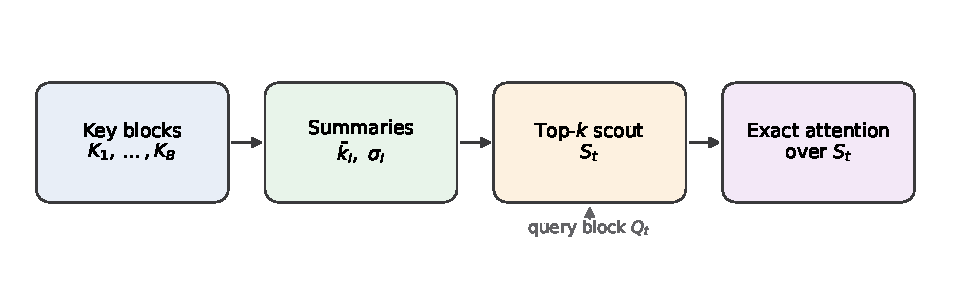
\includegraphics[width=0.9\linewidth]{figures/pipeline}
  \caption{The \textsc{Sieve} pipeline. Key blocks are summarised once per
  layer; each query block scores the summaries, keeps the top $k$, and reads
  only those keys and values.}
  \label{fig:pipeline}
\end{figure}

\subsection{Selection}
\label{sec:selection}

For a query block $Q_t$ we score every key block with the mean query
$\bar{q}_t$ and keep the best $k$:
\begin{equation}
  S_t = \topk{k}{\, s_1(\bar{q}_t), \dots, s_B(\bar{q}_t) \,} \cup \{\, t \,\} \cup G,
  \label{eq:selection}
\end{equation}
where the diagonal block $t$ preserves local context and $G$ is a small set of
global blocks (the first block and any block containing a separator token).

\subsection{Algorithm}

For each layer and each query block $t = 1, \dots, B$:
\begin{enumerate}
  \item Compute block summaries $\bar{k}_i$ and spreads $\sigma_i$
        (Equation~\eqref{eq:summary}); cache them across query blocks.
  \item Score the summaries and form $S_t$ with Equation~\eqref{eq:selection}.
  \item Gather the keys and values of the selected blocks:
        \begin{enumerate}
          \item copy the $|S_t|\,b$ keys into shared memory;
          \item stream the matching values in tiles of 128.
        \end{enumerate}
  \item Run exact attention over the gathered keys with an online softmax.
  \item Reuse $S_t$ for the next $r$ layers if the selections overlap by more
        than $90\%$.
\end{enumerate}

\subsection{Choosing the budget}

The budget $k$ trades accuracy for speed. We choose it per layer so that the
expected discarded mass stays below a tolerance $\varepsilon$:
\[
  k_\ell = \min \Bigl\{\, k : \E_{q}\bigl[\delta_\ell(S_k(q))\bigr] \le \varepsilon \Bigr\}.
\]
In practice $\varepsilon = 10^{-2}$ gives $k_\ell$ between 8 and 24 blocks.

\begin{description}
  \item[Scout cost] One matrix product of size $n/b \times B$ per layer.
  \item[Read cost] At most $(k + |G| + 1)\, b$ keys per query.
  \item[Memory] Linear in $m$; no attention matrix is ever materialised.
\end{description}

\section{Method}
\label{sec:method}

\textsc{Sieve} replaces the dense attention of every layer with a two-stage
operator: a \emph{scout} stage that scores block summaries, and a
\emph{read} stage that attends only to the blocks it selects.
Figure~\ref{fig:pipeline} shows the data flow.

\begin{figure}[t]
  \centering
  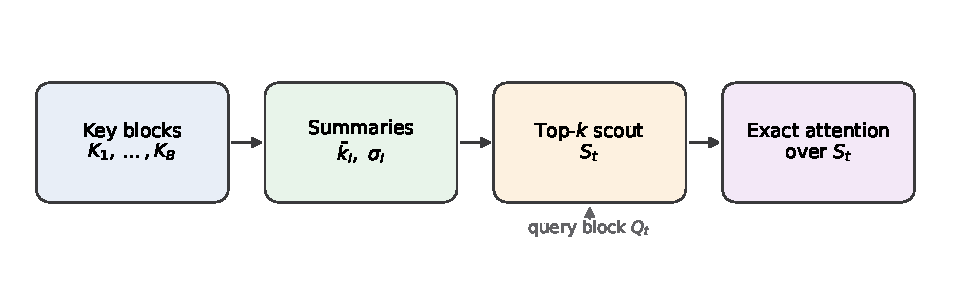
\includegraphics[width=0.9\linewidth]{figures/pipeline}
  \caption{The \textsc{Sieve} pipeline. Key blocks are summarised once per
  layer; each query block scores the summaries, keeps the top $k$, and reads
  only those keys and values.}
  \label{fig:pipeline}
\end{figure}

\subsection{Selection}
\label{sec:selection}

For a query block $Q_t$ we score every key block with the mean query
$\bar{q}_t$ and keep the best $k$:
\begin{equation}
  S_t = \topk{k}{\, s_1(\bar{q}_t), \dots, s_B(\bar{q}_t) \,} \cup \{\, t \,\} \cup G,
  \label{eq:selection}
\end{equation}
where the diagonal block $t$ preserves local context and $G$ is a small set of
global blocks (the first block and any block containing a separator token).

\subsection{Algorithm}

For each layer and each query block $t = 1, \dots, B$:
\begin{enumerate}
  \item Compute block summaries $\bar{k}_i$ and spreads $\sigma_i$
        (Equation~\eqref{eq:summary}); cache them across query blocks.
  \item Score the summaries and form $S_t$ with Equation~\eqref{eq:selection}.
  \item Gather the keys and values of the selected blocks:
        \begin{enumerate}
          \item copy the $|S_t|\,b$ keys into shared memory;
          \item stream the matching values in tiles of 128.
        \end{enumerate}
  \item Run exact attention over the gathered keys with an online softmax.
  \item Reuse $S_t$ for the next $r$ layers if the selections overlap by more
        than $90\%$.
\end{enumerate}

\subsection{Choosing the budget}

The budget $k$ trades accuracy for speed. We choose it per layer so that the
expected discarded mass stays below a tolerance $\varepsilon$:
\[
  k_\ell = \min \Bigl\{\, k : \E_{q}\bigl[\delta_\ell(S_k(q))\bigr] \le \varepsilon \Bigr\}.
\]
In practice $\varepsilon = 10^{-2}$ gives $k_\ell$ between 8 and 24 blocks.

\begin{description}
  \item[Scout cost] One matrix product of size $n/b \times B$ per layer.
  \item[Read cost] At most $(k + |G| + 1)\, b$ keys per query.
  \item[Memory] Linear in $m$; no attention matrix is ever materialised.
\end{description}

\section{Method}
\label{sec:method}

\textsc{Sieve} replaces the dense attention of every layer with a two-stage
operator: a \emph{scout} stage that scores block summaries, and a
\emph{read} stage that attends only to the blocks it selects.
Figure~\ref{fig:pipeline} shows the data flow.

\begin{figure}[t]
  \centering
  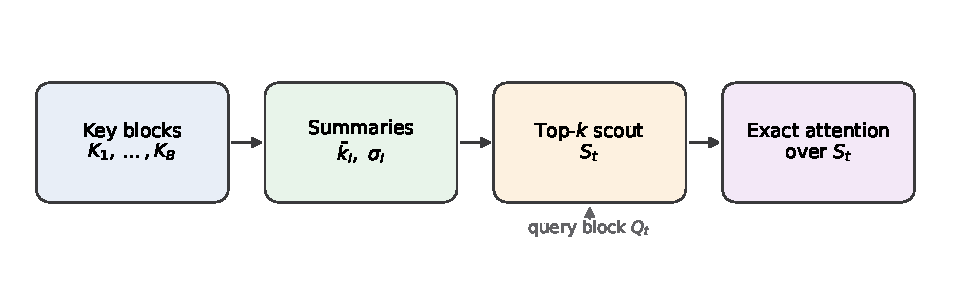
\includegraphics[width=0.9\linewidth]{figures/pipeline}
  \caption{The \textsc{Sieve} pipeline. Key blocks are summarised once per
  layer; each query block scores the summaries, keeps the top $k$, and reads
  only those keys and values.}
  \label{fig:pipeline}
\end{figure}

\subsection{Selection}
\label{sec:selection}

For a query block $Q_t$ we score every key block with the mean query
$\bar{q}_t$ and keep the best $k$:
\begin{equation}
  S_t = \topk{k}{\, s_1(\bar{q}_t), \dots, s_B(\bar{q}_t) \,} \cup \{\, t \,\} \cup G,
  \label{eq:selection}
\end{equation}
where the diagonal block $t$ preserves local context and $G$ is a small set of
global blocks (the first block and any block containing a separator token).

\subsection{Algorithm}

For each layer and each query block $t = 1, \dots, B$:
\begin{enumerate}
  \item Compute block summaries $\bar{k}_i$ and spreads $\sigma_i$
        (Equation~\eqref{eq:summary}); cache them across query blocks.
  \item Score the summaries and form $S_t$ with Equation~\eqref{eq:selection}.
  \item Gather the keys and values of the selected blocks:
        \begin{enumerate}
          \item copy the $|S_t|\,b$ keys into shared memory;
          \item stream the matching values in tiles of 128.
        \end{enumerate}
  \item Run exact attention over the gathered keys with an online softmax.
  \item Reuse $S_t$ for the next $r$ layers if the selections overlap by more
        than $90\%$.
\end{enumerate}

\subsection{Choosing the budget}

The budget $k$ trades accuracy for speed. We choose it per layer so that the
expected discarded mass stays below a tolerance $\varepsilon$:
\[
  k_\ell = \min \Bigl\{\, k : \E_{q}\bigl[\delta_\ell(S_k(q))\bigr] \le \varepsilon \Bigr\}.
\]
In practice $\varepsilon = 10^{-2}$ gives $k_\ell$ between 8 and 24 blocks.

\begin{description}
  \item[Scout cost] One matrix product of size $n/b \times B$ per layer.
  \item[Read cost] At most $(k + |G| + 1)\, b$ keys per query.
  \item[Memory] Linear in $m$; no attention matrix is ever materialised.
\end{description}

\section{Method}
\label{sec:method}

\textsc{Sieve} replaces the dense attention of every layer with a two-stage
operator: a \emph{scout} stage that scores block summaries, and a
\emph{read} stage that attends only to the blocks it selects.
Figure~\ref{fig:pipeline} shows the data flow.

\begin{figure}[t]
  \centering
  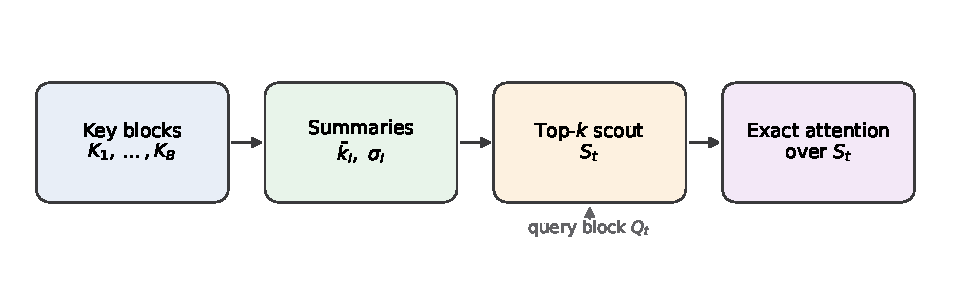
\includegraphics[width=0.9\linewidth]{figures/pipeline}
  \caption{The \textsc{Sieve} pipeline. Key blocks are summarised once per
  layer; each query block scores the summaries, keeps the top $k$, and reads
  only those keys and values.}
  \label{fig:pipeline}
\end{figure}

\subsection{Selection}
\label{sec:selection}

For a query block $Q_t$ we score every key block with the mean query
$\bar{q}_t$ and keep the best $k$:
\begin{equation}
  S_t = \topk{k}{\, s_1(\bar{q}_t), \dots, s_B(\bar{q}_t) \,} \cup \{\, t \,\} \cup G,
  \label{eq:selection}
\end{equation}
where the diagonal block $t$ preserves local context and $G$ is a small set of
global blocks (the first block and any block containing a separator token).

\subsection{Algorithm}

For each layer and each query block $t = 1, \dots, B$:
\begin{enumerate}
  \item Compute block summaries $\bar{k}_i$ and spreads $\sigma_i$
        (Equation~\eqref{eq:summary}); cache them across query blocks.
  \item Score the summaries and form $S_t$ with Equation~\eqref{eq:selection}.
  \item Gather the keys and values of the selected blocks:
        \begin{enumerate}
          \item copy the $|S_t|\,b$ keys into shared memory;
          \item stream the matching values in tiles of 128.
        \end{enumerate}
  \item Run exact attention over the gathered keys with an online softmax.
  \item Reuse $S_t$ for the next $r$ layers if the selections overlap by more
        than $90\%$.
\end{enumerate}

\subsection{Choosing the budget}

The budget $k$ trades accuracy for speed. We choose it per layer so that the
expected discarded mass stays below a tolerance $\varepsilon$:
\[
  k_\ell = \min \Bigl\{\, k : \E_{q}\bigl[\delta_\ell(S_k(q))\bigr] \le \varepsilon \Bigr\}.
\]
In practice $\varepsilon = 10^{-2}$ gives $k_\ell$ between 8 and 24 blocks.

\begin{description}
  \item[Scout cost] One matrix product of size $n/b \times B$ per layer.
  \item[Read cost] At most $(k + |G| + 1)\, b$ keys per query.
  \item[Memory] Linear in $m$; no attention matrix is ever materialised.
\end{description}
